% !TEX encoding = UTF-8 Unicode
\documentclass[a4paper]{article}

\usepackage{color}
\usepackage{url}
\usepackage[T2A]{fontenc} % enable Cyrillic fonts
\usepackage[utf8]{inputenc} % make weird characters work
\usepackage{graphicx}

%\usepackage[english,serbian]{babel}
\usepackage[english,serbianc]{babel} %ukljuciti babel sa ovim opcijama, umesto gornjim, ukoliko se koristi cirilica

\usepackage[unicode]{hyperref}
\hypersetup{colorlinks,citecolor=green,filecolor=green,linkcolor=blue,urlcolor=blue}

\usepackage{listings}
\usepackage{amsmath}

\newtheorem{primer}{Пример}[section] %ćirilični primer
% \newtheorem{primer}{Primer}[section]

\definecolor{mygreen}{rgb}{0,0.6,0}
\definecolor{mygray}{rgb}{0.5,0.5,0.5}
\definecolor{mymauve}{rgb}{0.58,0,0.82}

\lstset{ 
  backgroundcolor=\color{white},   % choose the background color; you must add \usepackage{color} or \usepackage{xcolor}; should come as last argument
  basicstyle=\scriptsize\ttfamily,        % the size of the fonts that are used for the code
  breakatwhitespace=false,         % sets if automatic breaks should only happen at whitespace
  breaklines=true,                 % sets automatic line breaking
  captionpos=b,                    % sets the caption-position to bottom
  commentstyle=\color{mygreen},    % comment style
  deletekeywords={...},            % if you want to delete keywords from the given language
  escapeinside={\%*}{*)},          % if you want to add LaTeX within your code
  extendedchars=true,              % lets you use non-ASCII characters; for 8-bits encodings only, does not work with UTF-8
  firstnumber=1000,                % start line enumeration with line 1000
  frame=single,	                   % adds a frame around the code
  keepspaces=true,                 % keeps spaces in text, useful for keeping indentation of code (possibly needs columns=flexible)
  keywordstyle=\color{blue},       % keyword style
  language=Python,                 % the language of the code
  morekeywords={*,...},            % if you want to add more keywords to the set
  numbers=left,                    % where to put the line-numbers; possible values are (none, left, right)
  numbersep=5pt,                   % how far the line-numbers are from the code
  numberstyle=\tiny\color{mygray}, % the style that is used for the line-numbers
  rulecolor=\color{black},         % if not set, the frame-color may be changed on line-breaks within not-black text (e.g. comments (green here))
  showspaces=false,                % show spaces everywhere adding particular underscores; it overrides 'showstringspaces'
  showstringspaces=false,          % underline spaces within strings only
  showtabs=false,                  % show tabs within strings adding particular underscores
  stepnumber=2,                    % the step between two line-numbers. If it's 1, each line will be numbered
  stringstyle=\color{mymauve},     % string literal style
  tabsize=2,	                   % sets default tabsize to 2 spaces
  title=\lstname                   % show the filename of files included with \lstinputlisting; also try caption instead of title
}

\begin{document}

\title{Генетичко програмирање\\ \small{Семинарски рад у оквиру курса\\Методологија стручног и научног рада\\ Математички факултет}}

\author{Александра Стојановић, Ивана Ивановић,\\ Александар Стефановић, Оливера Поповић\\ mi16048@alas.matf.bg.ac.rs, mi16120@alas.matf.bg.ac.rs,\\ ai16222@alas.matf.bg.ac.rs, mi16064@alas.matf.bg.ac.rs}

%\date{9.~april 2015.}

\maketitle

\abstract{
U ovom tekstu je ukratko prikazana osnovna forma seminarskog rada. Obratite pažnju da je pored ove .pdf datoteke, u prilogu i odgovarajuća .tex datoteka, kao i .bib datoteka korišćena za generisanje literature. Na prvoj strani seminarskog rada su naslov, apstrakt i sadržaj, i to sve mora da stane na prvu stranu! Kako bi Vaš seminarski zadovoljio standarde i očekivanja, koristite uputstva i materijale sa predavanja na temu pisanja seminarskih radova. Ovo je samo šablon koji se odnosi na fizički izgled seminarskog rada (šablon koji \emph{morate} da koristite!) kao i par tehničkih pomoćnih uputstava. Pročitajte tekst pažljivo jer on sadrži i važne informacije vezane za zahteve obima i karakteristika seminarskog rada.}

\tableofcontents

\newpage

\section{Увод}

Генетичко програмирање је метода која је настала као један од покушаја да се спроведе аутоматизација прављења рачунарских програма за решавања проблема задатих на веома апстрактном нивоу. Основни циљ је да ови проблеми буду тако дефинисани да је познато једино шта треба да буде урађено, без додатних информација о форми или структури решења. Да би машине на овај начин радиле посао који иначе ради човек, потребно је да оне искажу неки вид интелигенције. Међу првима је постојање овог проблема поменуо Алан Тјуринг у свом раду о интелигентним машинама из 1948. године \cite{turing}.


\section{Историјат}
Први запис предлога за развијање програма вероватно је запис Алана Тјуринга из 1950. године. Дошло је до размака од 25 година пре објављивања књиге „Прилагођавање природним и вештачким системима“ Џона Холанда, која је поставила теоријске и емпиријске темеље науке.
Џон Холанд постао је познат по генетском алгоритму, али о програмима је већ говорио у свом семинарском раду из 1962. године. Дуго се сматрало да излагање рачунарских програма
случајним силама мутације и рекомбинације неће донети одрживе програме. Сматрало се да је рачунарски код сувише слаб да би се могао побољшати случајним генерисањем у еволуцији.
Појам генетско програмирање описује истраживачко подручје у пољу еволуцијског рачунања које се бави еволуцијом рачунарског кода. Њени алгоритми имају за циљ да олакшају решења проблема машинског учења или да индукују прецизна решења у облику граматички исправних (језичких) структура за аутоматско програмирање рачунара. На структуре које одређују понашање рачунара се примењује општи поступак приказан на слици \ref{fig:kontrola_toka}.


Дуга је прошло док није утврђено  да није немогуће еволуирати рачунарски код.о времен Овај развој захтевао је неколико различитих (мањих) посредних корака. Пре свега оригиналне генетске алгоритме који користе низове битова фиксне дужине да представе бројеве у проблемима оптимизације. Прво схватање било је да се систем правила, уместо бројева који представљају проблематична решења, може подвргнути еволуцији. У другом семинарском раду, Холанд и Реитман представили су систем класификатора који је омогућио да се правила развију током еволуције. Кључни допринос система класификатора будућем пољу генетског програмирања је био да су сва правила знак обележја програмских језика и извршавања сложенијих рачунарских кодова.


Убрзо након Холанда и Реитмана, Смит је увео репрезентацију променљиве дужине.  Омогућио је да се уједине правила у програме засноване на правилима који могу да реше задатак дефинисан функцијом прилагођености, o којој ће бити више речи у наредном поглављу \ref{fitness}. Ричард Форсит је 1981. године демонстрирао успешну еволуцију малих програма, представљених као дрвеће, за извршење класификације доказа о месту злочина за матичну канцеларију у Великој Британији. Форсит је објавио логички систем правила с параметрима који нам омогућавају класификацију примера у различите класе. За обучавање класификатора се користи низ обука узорака. Програми би логички и нумерички процењивали узорке података да би добили закључке о класи примера.\cite{genetic_algorithms}


У другој половини 1980-их, број раних ГП система се повећавао. Kрамер је 1985. представио два еволуциона програмска система заснована на различитим једноставним језицима. Хиклин, Фујики и Дикинсон написали су системе који представљају претече за одређене апликације користећи стандардни програмски језик Лисп, а Коза је 1989. коначно документовао методу која је користила универзални језик и примењена је на много различитих проблема. Гeнетско програмиранје је наставило са напредовањен објављивањем књиге Џона Козе 1992. године. Коза је објавио серију од 4 књиге, почев од 1992. године са пратећим видео снимцима. Након тога, дошло је до огромног повећања броја публикација са Библиографијом о генетском програмирању, премашивши 10 000 уноса.


Коза је 1996. започеo годишњу конференцију о генетском програмирању  коју је 1998. пратила годишња конференција ЕуроГП, и прва књига у ГП серији коју је уредио Коза. 1998. године представљен је и први уџбеник ГП-а. Рик Риоло је наставио процват ГП-а, што је довело до првог специјалистичког часописа опште праксе, а три године касније, 2003. године основана је годишња радионица „Теорије и праксе генетичког програмирања“. Радови о генетском програмирању и даље се објављују на различитим конференцијама и повезаним часописима. Данас постоји деветнаест ГП књига укључујући неколико књига за студенте.

\section{Опис алгоритма}

Идеја на којој генетичко програмирање почива је процес еволуције који се јавља у природи. Самим тим то је техника која спада у групу алгоритама  \textbf{еволутивног израчунавања} \cite{compIntelligence}. Еволуција подразумева промену особина укупне популације кроз више смењених генерација. Постојало је током времена више теорија еволуције, док је данас опште прихваћена теорија чији је творац британски биолог Чарлс Дарвин. По његовој теорији, сви живи организми се развијају процесом природне селекције \cite{darwin1859}. Тим процесом јединке које су боље прилагођене имају већу вероватноћу да преживе и да оставе потомство, које је углавном једнако или чак и боље прилагођено од родитеља. Захваљујући томе што ћелије сваког живог бића садрже хромозоме, који су сачињени од гена, они могу да оставе потомство. Ген је основна јединица наслеђивања, која преноси поруке из генерације у генерацију. Дакле, репродукција подразумева комбинацију гена родитеља уз мале количине мутације. Карактеристике, односно генетски материјал прилагођенијих јединки углавном опстаје кроз генерације и у неком тренутку почиње да доминира, док остале карактеристике најчешће ишчезну.\newline

У овом одељку биће описано како се процес еволуције осликава на генетичко програмирање, које су његове основне компоненте као и то које одлуке треба донети при прилагођавању алгоритма задатом проблему.

\subsection{Општи алгоритам}

У генетичком програмирању популацију чине рачунарски програми. Еволуцијом се од почетних, најчешће на случајан начин генерисаних програма, добијају нови, у нади бољи и ефикаснији програми. Обзиром да је то случајан процес, резултат никада не може бити гарантован. Ипак, управо та случајност даје могућност превазилажења неких проблема које имају други детерминистички алгоритми \cite{fieldGuidetoGP}. На слици \ref{fig:kontrola_toka} приказан је дијаграм контроле тока опште верзије алгоритма. У наставку биће детаљно описан сваки од наведених корака алгоритма.

\begin{figure}[h!]
    \begin{center}
        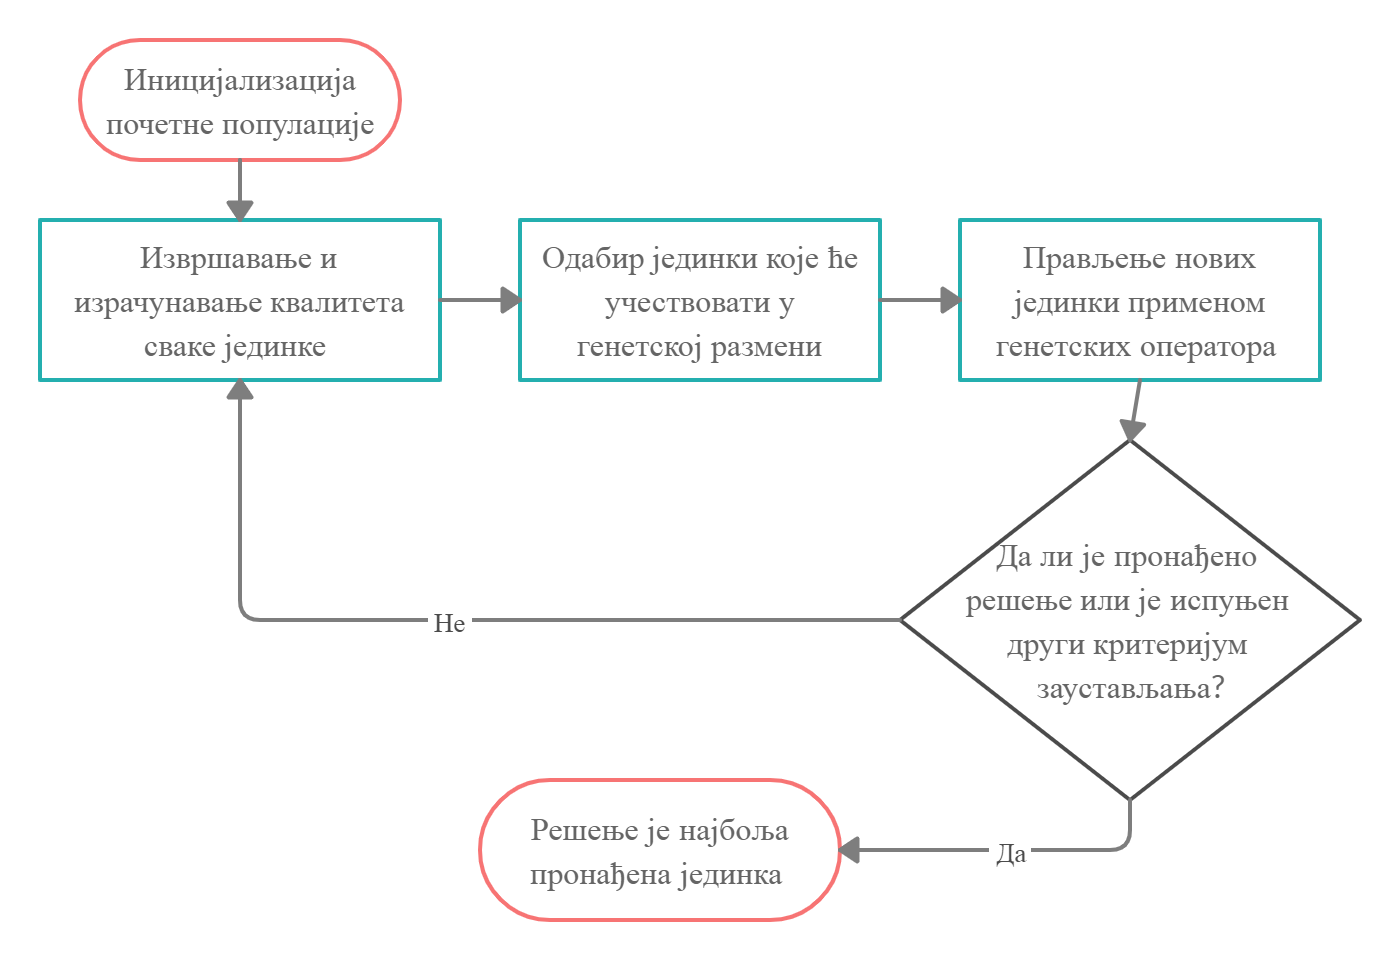
\includegraphics[scale=0.22]{opsti_algoritam.png}
    \end{center}
    \caption{Општи алгоритам генетичког програмирања}
    \label{fig:kontrola_toka}
\end{figure}

\bigskip
\noindent
\textbf{\large Репрезентација јединки}\newline

У генетичком програмирању, јединке су заправо рачунарски програми који се могу извршавати. Иако то на први поглед делује логично, оне неће бити представљене линијама кода. Разлог томе је што је неопходно да над изабраном репрезентацијом буду дефинисани генетски оператори, тако да извршавање буде ефикасно. Репрезентација која то испуњава је она у виду \textbf{синтаксних стабала} \cite{synTrees}.\newline

Код синтаксних стабала, основно је да се променљиве и константе налазе у листовима (најнижи чворови) и називају се терминалима, док се у осталим чворовима налазе функције. Функције могу бити различите природе, на пример аритметичке, тригонометријске или логичке, али могу бити и различите програмске конструкције попут условних израза и петљи. Свако овакво стабло мора имати скуп дефинисаних терминала и функција који заједно чине такозвани \textbf{примитивни скуп} генетичког програмирања. 

\begin{primer}
    Нека је проблем задат аритметичком формулом: 
    \begin{equation} 
        \label{eq:sintaksno_stablo}
        2*\pi-\frac{5+x}{y-4}
    \end{equation}
    Одговарајући скуп терминала: \{2, $\pi$, 5, x, y, 4\}, скуп функција:\newline \{+, -, *, /\}, док је одговарајуће синтаксно стабло дато на слици \ref{fig:sintaksno_stablo}.

    \begin{figure}[h!]
        \begin{center}
        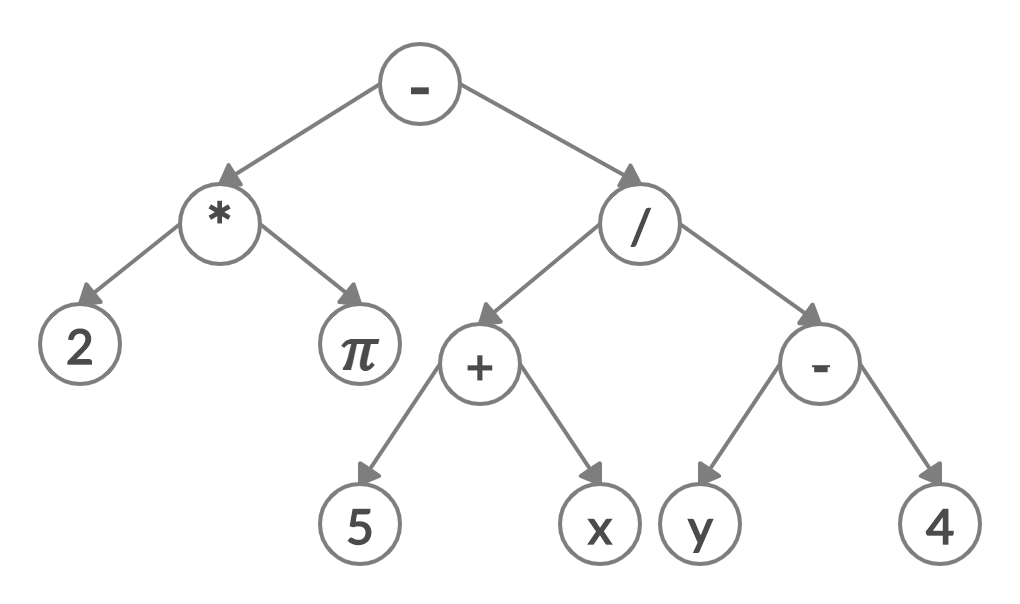
\includegraphics[scale=0.22]{sintaksno_stablo.png}
        \end{center}
        \caption{Синтаксно стабло које одговара формули \eqref{eq:sintaksno_stablo}}
        \label{fig:sintaksno_stablo}
    \end{figure}
\end{primer}

\medskip
Репрезентација стаблима има неколико импликација које треба имати на уму \cite{compIntelligence}:
\begin{itemize}
    \item Величина (висина), облик (какве су гране чворова) и сложеност јединки нису фиксирани, већ се могу разликовати. Те особине се чак и код једне јединке могу мењати током времена, услед примене оператора за репродукцију.
    \item За сваки проблем посебно се мора дефинисати примитивни скуп. Као додатак, могу бити дефинисана и семантичка правила која обезбеђују конструкцију исправних стабала. На пример: \newline
    \emph{Делилац никада не сме да буде једнак 0.}
\end{itemize}

\bigskip
\noindent
\textbf{\large Иницијализација популације}\newline

Генерисање почетне популације обично се врши на случајан начин. Притом се поштују сва дефинисана ограничења, уколико она постоје. Две најстарије и најједноставније методе су \textbf{потпуна метода} (eng.~{\em full method}) и \textbf{метода раста} (eng.~{\em grow method}), док се често користи и њихова пола-пола комбинација \cite{fieldGuidetoGP}. \newline

Прва метода зове се потпуна јер креира потпуна стабла. Стабло је потпуно уколико су му сви листови на истој дубини. \textbf{Дубина чвора} представља број грана које треба прећи да би се од корена дошло до тог чвора. \emph{Дубина чвора са вредношћу $\pi$ приказаног на слици \ref{fig:sintaksno_stablo} износи \underline{2}}. По потпуној методи, вредности у чворовима се бирају на случајан начин из скупа функција све док се не дође до максималне дубине. Максимална дубина је један од унапред задатих параметара. Након тога се на случајан начин вредности бирају из скупа терминала. По другој методи, методи раста, чворови се бирају на случајан начин из целог примитивног скупа док се не дође до максималне дубине, а након тога се такође бирају само терминали. Основна разлика између ове две методе је што метода раста дозвољава креацију стабала са више различитих величина и облика.\newline

Ипак, ниједна од ове две методе не пружа довољно велику разноврсност. Због тога се данас нашироко користи њихова комбинација коју је 1992. предложио Џон Коза \cite{koza}. Она подразумева да се прва половина генерације креира коришћењем потпуне методе, а друга методом раста.\newline

\bigskip
\noindent
\textbf{\large Функција прилагођености}\newline 
\label{fitness}

Функција прилагођености (eng.~{\em fitness function}) даје оцену \textbf{квалитета јединке}. Она треба да буде одабрана тако да може да се израчуна за сваку јединку а да израчунавање притом буде што ефикасније \cite{vi}. Зависи од проблема који се решава, али се у генетичком програмирању најчешће реализује тако што постоји скуп тест случајева којима се свака јединка евалуира. То значи да постоји одређени број улаза за које се знају очекивани излази, па се евалуира колико излаза је јединка, односно програм погодио.
Осим као мера квалитета јединке, функција прилагођености се такође може користити да додели пенале оним јединкама које нису прихватљиве или нису семантички тачне.\newline


\bigskip
\noindent
\textbf{\large Селекција}\newline

Селекција се користи како би се пронашле боље прилагођене јединке које ће учествовати у репродукцији. То се врши коришћењем функције прилагођености. На основу њене вредности јединке се узимају са одређеном вероватноћом. Најчешће се користе \textbf{турнирска селекција} и селекција пропорционала вредности функције прилагођености, али се могу користити и друге селекционе методе еволутивног израчунавања \cite{compIntelligence}. Код турнирске селекције бира се одређени број јединки из популације, на случајан начин. Оне се упоређују и бира се најбоља од њих. Она ће учествовати у репродукцији. Постоје и разне друге варијанте турнирске селекције, али је њена предност у сваком случају то што и средње квалитетне јединке могу добити прилику да оставе потомство. Пример селекције пропроционалне вредности функције прилагођености је \textbf{рулетска селекција} (eng.~{\em roulette wheel selection}). По њој, вероватноћа да ће јединка бити изабрана једнака је: 
\begin{equation} 
    p_i = \frac{f(i)}{\sum_{j}^{N} f(i)}
\end{equation}
где је f(i) вредност функције прилагођености јединке i, док је N укупан број јединки у популацији \cite{vi}.\newline


\bigskip
\noindent
\textbf{\large Репродукција}\newline

Репродукција представља начин на који се од два селекцијом изабрана родитеља добијa потомство. Код генетичког програмиранја најчешће се користи метод укрштања подстабала. На случајан начин одаберу се тачке укрштања код оба родитеља, након чега се једноставно замене подстабла родитеља са кореном у тачки укрштања. Постоје две опције, креирање једног или два детета разменом. Проблем код овог метода је то што се најчешће барата са стаблима код којих сваки чвор има најмање двоје деце, што доводи до тога да већи број чворова припада скупу терминала. Последица тога је што се размењују мање количине генетског материјала, јер се чешће на случајан начин погоди управо неки од терминала. Да би се избегао овај проблем, Коза је 1992. предложио нашироко коришћен приступ бирања функција 90\% времена, а листова преосталих 10\%. Постоји још много видова репродукције који се користе код генетичког програмирања \cite{fieldGuidetoGP}.\newline

\bigskip
\noindent
\textbf{\large Мутација}\newline

Мутација се примењује како током времена јединке не би постале сувише сличне. Такође помаже у избегавању локалних екстремума, у ком би се највероватније јединке заглавиле уколико не би било мутације.
Мутација се најчешће имплементира тако да се на случајан начин изабере тачка јединке, па се подстабло са кореном у тој тачки замени случајно генерисаним стаблом. Још један чест начин имплементације је да се такође на случајан начин изабере тачка у стаблу јединке, али се сада вредност у том чвору замени случајно одабраном вредношћу исте арности из примитивног скупа. Ако нема других примитива исте арности чвор се не дира. 

Основна разлика ове две имплементације је у примени. Примена прве подразумева мутацију тачно једног подстабла, док се код друге обично она примени на сваки чвор са одређеном вероватноћом што омогућава да више чворова буде мутирано. \newline

Избор који ће се од оператора (укрштање или мутација) применити врши се са одређеном вероватноћом, која се задаје као параметар алгоритма. У генетичком програмирању оператори су обично ексклузивни, што значи да се примењује укрштање или мутација.

\subsection{Прилагођавање алгоритма}

Генетичко програмирање у свом основном облику не користи специфичности ниједног проблема, те се може применити на широк спектар различитих проблема. Међутим, да би се могао користити за решавање неког конкретног проблема потребно га је прилагодити. Одлуке које притом треба донети \cite{fieldGuidetoGP}:\newline

\textbf{1. Како изгледа примитивни скуп?}\newline
Примитивни скуп треба да буде дефинисан тако да је могуће изразити решење коришћењем садржаних примитива. Нажалост, врло често није могуће предвидети примитивни скуп тако да задовољава ово својство. Ипак, захваљујући природи генетског програмирања, врло често иако решење не може да се представи, алгоритам може развити програме који представљају његову апроксимацију. То је најчешће и сасвим довољно. Примери функција дати су у табели \ref{tab:primitive}. \newline
    
\begin{table}[h!]
    \begin{center}
    \caption{Пример функција генетичког програмирања.}
    \medskip
        \begin{tabular}{|c|c|} 
        \hline 
        природа функције & примери\\[0.3em] \hline 
        аритметичка & +, -, $\times$, $\div$\\[0.3em]
        математичка & sin, cos, exp\\[0.3em]
        логичка & $\land$, $\lor$, $\not$\\[0.3em] 
        условни изрази & if-else\\[0.3em] 
        петље & for, while\\[0.3em] 
        \hline
        \end{tabular}
    \label{tab:primitive}
    \end{center}
\end{table}
    
\textbf{2. Како изгледа функција прилагођености?}\newline
Квалитет, односно прилагођеност јединке може се рачунати на разне начине, а то који ће се користити зависи од природе проблема. На пример може се рачунати као грешка између излаза и жељеног излаза, као тачност у класификацији објеката или као растојање од жељеног резултата.\newline

\textbf{3. Који ће параметри бити коришћени?}\newline
Пре покретања алгоритма потребно је подесити неколико параметара, међу којима су величина популације, вероватноће примене оператора, максимална величина програма и слични детаљи. Иако вредности ових параметара зависе од проблема, генетско програмирање је у пракси углавном веома моћно те ће више параметара дати задовољавајуће резултате. Због тога постоје неке препоруке од којих вредности кренути. Правило је да величина популације буде највећа са којом систем који користимо може да ради, а да је то најмање 500. Укрштање се обично примењује са највећом вероватноћом, која је 90\% или више. Насупрот томе, мутација се обично примењује са веома малом вероватноћом, обично око 1\%. Вероватноћа мутације је обично толико мала јер би у супротном алгоритам брзо прерастао у случајну претрагу услед превише измена.\newline

\textbf{4. Који ће бити критеријум заустављања?}\newline
Као критеријум заустављања најчешће се користи унапред дефинисан максималан број генерација. Овај број не треба да буде велики. Поред тога може бити дефинисан још и неки предикат успеха који је специфичан за проблем који се решава. Такође, извршавање се обично прекида уколико се пронађе решење које задовољава проблем. Као резултат на крају извршавања најчешће се узима најбоља пронађена јединка до тог тренутка. \newline

\section{Примери примене}
Примена генетичког програмирања у индустрији је разнолика и рапидно се повећава годинама. Биће речи о неким од важнијих или занимљивих радова написаних о изабраним дисциплинама, што не значи да не постоји доста радова, односно симулација зарад решавања других проблема у разним другим дисциплинама.
\subsection{Роботика}
Један од проблема који се симулира јесу два робота који играју познату игру јурке. Оба робота/играча поседују информацију о томе ко јури и где му се апроксимативно налази противник. Циљ игре је што краће бити онај који треба да јури противника. Играју се четири рунде од којих се свака састоји од 25 симулација. Улоге се, у току једне рунде, мењају кад онај који јури буде од свог противника на дужини од једног возила. Играчев резултат за ту рунду рачуна се као број колико пута није био онај који јури подељен са 25. \cite{tag}

Такође, постоји и проблем навигације робота како би нашао храну која је постављена дуж неправилне линије; где робот зна да извршава примитивне операције: померање напред, окретање лево/десно као и "мирисање" хране.
Овај проблем решен је уз помоћ програмског језика Lisp и коришћењем с-израза. \cite{lisp} Путање које су коришћене су следеће:
\begin{itemize}
	\item "Santa Fe" путања (приказана на слици \ref{fig:santa_fe}) - направљена од 89 комада хране, где између њих постоји једна, две или три празнине без хране који могу бити и на угловима линије кретања робота
	\item "Los Altos Hills" путања - састављена од 157 комада хране, где 105. комад представља 89. комад односно крај из претходне путање. Након тог комада, додате су још две ирегуларности у путањи:
	\begin{itemize}
		\item[$-$] налажење хране два места лево или десно од претходног комада хране; прво појављивање после 116. комада хране 
		\item[$-$] померање једно место унапред, затим проналажење хране два месте лево или десно; прво појављивање после 136. комада хране
	\end{itemize}
\end{itemize}

\begin{figure}[h!]
    \begin{center}
        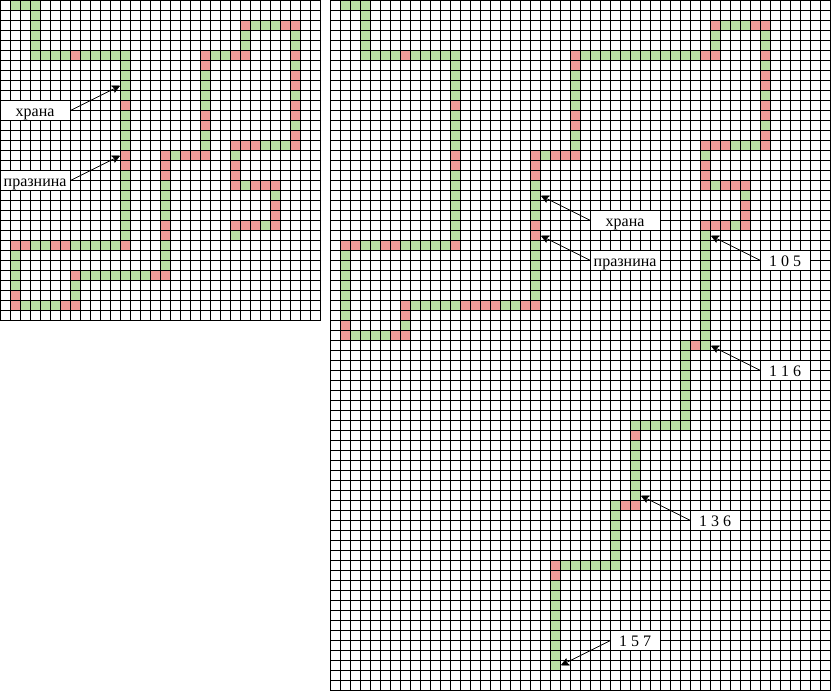
\includegraphics[scale=0.45]{santa_fe.png}
    \end{center}
    \caption{Изглед "Santa Fe" путање}
    \label{fig:santa_fe}
\end{figure}

За прву путању успешно је решен проблем у 21. генерацији, док је за другу путању било потребно стићи до 19. генерације. \cite{koza} 
\subsection{Медицина}
Иако генетичко програмирање не може бити једино решење када се анализирају биолошки подаци, оно је важно као додатан аналитички алат који има потенцијал да пружи изненађујуће и непредвидиве резултате. Способност да пронађе корисне комбинације својстава и да их прикаже у облику разумљивом за људе га чине погодним за истраживање болести попут рака. \cite{cancer}

Коришћење унапређеног генетичког програмирања је показало боље резултате у проблему класификације података од класичних алгоритама машинског учења попут линеарне регресије, неуронских мрежа и класификације базиране на суседима. \cite{egp}
\subsection{Економија}
Можда једна од најбитнијих проблема са којима се сусреће ова дисциплина је предвиђање банкрупта компанија. Коришћењем генетичког програмирања дошло се до занимљивих карактеристика података ових предузећа. \cite{bankruptcy}

Такође, у економији је од велике важности предвидети податке на тржиштима хартија од вредности (берзама), како због смањења губитака од куповине и продаје акција, тако и зарад максимизовања профита. \cite{stock}

\section{Мета-генетичко програмирање}

Мета-генетичко програмирање подразумева упоредно еволуирање програма који врши генетичко програмирање, које замењује ручно подешавање параметара и одлика алгоритма.


Постоје различити начини да се примени мета-генетичко програмирање. Према подели датој у \cite{edmonds2001meta} то су:

\begin{itemize}
	\item Они који додају додатни генетички материјал у геном,
	\item Они који праве колекције модула и имплицитно мењају \emph{језик} изражавања гена,
	\item Они који мењају фиксни скуп параметара, попут параметра учесталости мутације
	\item Они који еволуирају операторе генетичког програмирања, тако да се не користе фиксни, унапред-познати оператори.
\end{itemize}

У даљем тексту ће пажња бити посвећена последњем начину. Треба узети у обзир да мета-генетички алгоритми изискују знатно више рачунарских ресурса, јер сада свака јединка на првом мета-нивоу сада захтева извршавање алгоритма генетичког програмирања, ради израчунавања њене прилагођености, и сходно томе, треба проценити да ли је додатно улагање ресурса вредно могућих добитака.

\subsection{Еволуирање оператора генетичког алгоритма}

Обично су оператори генетичког програмирања унапред задати и фиксни, и најчешће се ради о комбинацији укрштања и мутација, али су истраживани и неки алтернативни оператори, и испоставља се да у неким случајевима, коришћење тих алтернативних оператора, заједно са ,,уобичајеним'' операторима даје боље резултате. Дакле, паметним одабиром и укључивањем одређених оператора мутације, могуће је постићи бољи учинак програма који врши генетичко програмирање.


Међутим, одабир оператора није тривијалан, јер је могуће да неки јако добар оператор не буде ни лак за тумачење, ни интуитиван, односно, мало је вероватно да би нека особа сама осмислила такав оператор, што сасвим одговара мотивацији генетичких алгоритама уопште, где је простор претраге јако велик, и посао проналажења решења је препуштен рачунару, а не особи.


Као и у типичном генетичком програмирању, јединке се приказују помоћу синтаксних стабала, с тим што оваква стабла садрже инструкције које представљају операторе мутације. У овом случају, прилагођеност је сразмерна прилагођености јединки које јединка мета-генетичког програмирања може да генерише својим извршавањем. 


\subsubsection{Елементи оператора}
У \cite{edmonds2001meta}, коришћени су ови листови:
\begin{itemize}
\item \texttt{rand1} — Вратити прво стабло, са насумично изабраним чвором
\item \texttt{rand2} — Вратити друго стабло, са насумично изабраним чвором
\item \texttt{bott1} — вратити прво стабло, са изабраним кореним чвором
\item \texttt{bott2} — вратити друго стабло, са изабраним кореним чвором
\end{itemize}

И следећи унутрашњи чворови:

\begin{itemize}
\item \texttt{top} — одсећи део стабла тако да изабрани чвор сада постане нови корен
\item \texttt{up1} — вратити исто дрво, али променити изабрани чвор са тренутног на његово прво дете (ако такво не постоји, вратити неизмењено дрво)
\item \texttt{up2} — вратити исто дрво, али променити изабрани чвор са тренутног на његово друго дете (ако такво не постоји, вратити неизмењено дрво)
\item \texttt{down} — вратити исто дрво, али променити изабрани чвор са тренутног на његовог родитеља (ако родитељ не постоји, вратити неизмењено дрво) 
\item \texttt{down1} — исто као \texttt{down} (како оператори не би имали склоност према \texttt{up} операторима)
\item \texttt{subs} — вратити дрво које је први аргумент, тако да је његов изабрани чвор замењен дрветом које је други аргумент.
\end{itemize}

На пример, оператор који има структуру задату сликом \ref{fig:mgp_primer} се може тумачити као "прво дете корена првог стабла замени са другим стаблом и вратити тако добијено стабло''.

\begin{figure}[h!]
    \begin{center}
    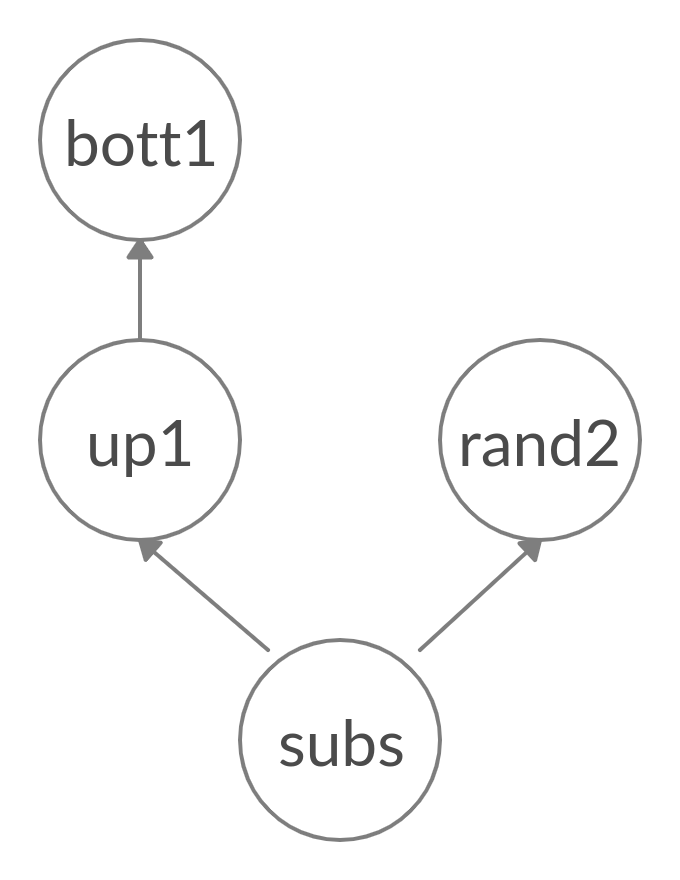
\includegraphics[scale=0.12]{mgp_primer.png}
    \end{center}
    \caption{Пример једног оператора}
    \label{fig:mgp_primer}
\end{figure}

% UPUTSTVA
% Vaš seminarski rad mora da sadrži najmanje jednu \textbf{sliku}, najmanje jednu \textbf{tabelu} i najmanje \textbf{sedam referenci} u spisku literature. Najmanje jedna slika treba da bude originalna i da predstavlja neke podatke koje ste Vi osmislili da treba da prezentujete u svom radu. Isto važi i za najmanje jednu tabelu. 	Od referenci, neophodno je imati bar jednu \textbf{knjigu}, bar jedan \textbf{naučni članak} iz odgovarajućeg časopisa i bar jednu adekvatnu \textbf{veb adresu}. 
% \textbf{Dužina seminarskog rada treba da bude od 10 do 12 strana.} Svako prekoračenje ili potkoračenje biće kažnjeno sa odgovarajućim brojem poena. Eventualno, nakon strane 12, može se javiti samo tekst poglavlja \textbf{Dodatak} koji sadrži nekakav dodatni k\^{o}d, ali je svakako potrebno da rad može da se pročita i razume i bez čitanja tog dodatka. 

% TABELA
% \begin{table}[h!]
% \begin{center}
% \caption{Razlčita poravnanja u okviru iste tabele ne treba koristiti jer su nepregledna.}
% \begin{tabular}{|c|l|r|} \hline
% centralno poravnanje& levo poravnanje& desno poravnanje\\ \hline
% a &b&c\\ \hline
% d &e&f\\ \hline
% \end{tabular}
% \label{tab:tabela1}
% \end{center}
% \end{table}

% KOD
% Za ubacivanje koda koristite paket \textbf{listings}:
% \url{https://en.wikibooks.org/wiki/LaTeX/Source_Code_Listings}
% 
% 
% \begin{lstlisting}[caption={Primer ubacivanja koda u tekst},frame=single, label=simple]
% # This program adds up integers in the command line
% import sys
% try:
%     total = sum(int(arg) for arg in sys.argv[1:])
%     print 'sum =', total
% except ValueError:
%     print 'Please supply integer arguments'
% \end{lstlisting}


\section{Закључак}
\label{sec:zakljucak}

Од првог коришћења генетскг програмирања 1990. године, рачунска снага се повећала за фактор од 40 000 по Моореовом закону сваких 18 месеци.Како Коза истиче, иако су у почетку били доступни само проблеми са играчкама кроз генетско програмирање, касније повећање рачунске снаге и методолошког напретка генетског програмирања омогућила су нова решења патентираних изума, као и потпуно нове проналаске који су сами по себи патентирани .

\addcontentsline{toc}{section}{Литература}
\appendix
\bibliography{literatura} 
\bibliographystyle{plain}

\appendix
\section{Додатак}
Ovde pišem dodatne stvari, ukoliko za time ima potrebe.
Ovde pišem dodatne stvari, ukoliko za time ima potrebe.
Ovde pišem dodatne stvari, ukoliko za time ima potrebe.
Ovde pišem dodatne stvari, ukoliko za time ima potrebe.
Ovde pišem dodatne stvari, ukoliko za time ima potrebe.


\end{document}
